\section*{CHAPTER 1. ABC}
\addcontentsline{toc}{section}{\numberline{}CHAPTER 1. ABC}
\setcounter{section}{1}
\setcounter{subsection}{0}
\setcounter{figure}{0}
\setcounter{table}{0}

\subsection{How to use latex}

\subsubsection{Table making}

    \begin{table}[H]
        \centering
        \caption{Experiment results}
        \begin{tabularx}{0.85\textwidth}{
            | >{\centering}y%\arraybackslash}y
            | >{\centering\arraybackslash}a
            | >{\centering\arraybackslash}a
            | >{\centering\arraybackslash}y|
            }
                \hline
            \bfseries  No.   &\bfseries Voltage \hspace{1cm}(mV)   &\bfseries Reference \hspace{0pt} (mV)  & \bfseries Error \hspace{0pt}(\%)\\\hline
             1  &   &   &\\\hline
             2  &   &   &\\\hline
             3  &   &   &\\\hline
        ...  &   &   &\\\hline
        \end{tabularx}
            \label{bang31}
    \end{table}

\subsubsection{Equation}
    \begin{equation}\label{pt31}
        F(x) = \int^a_b \frac{1}{3}x^3
    \end{equation}
    
Equation \ref{pt31} is an example of an integral equation.

\subsubsection{Add figure}
\begin{figure}[h!]
    \centering
    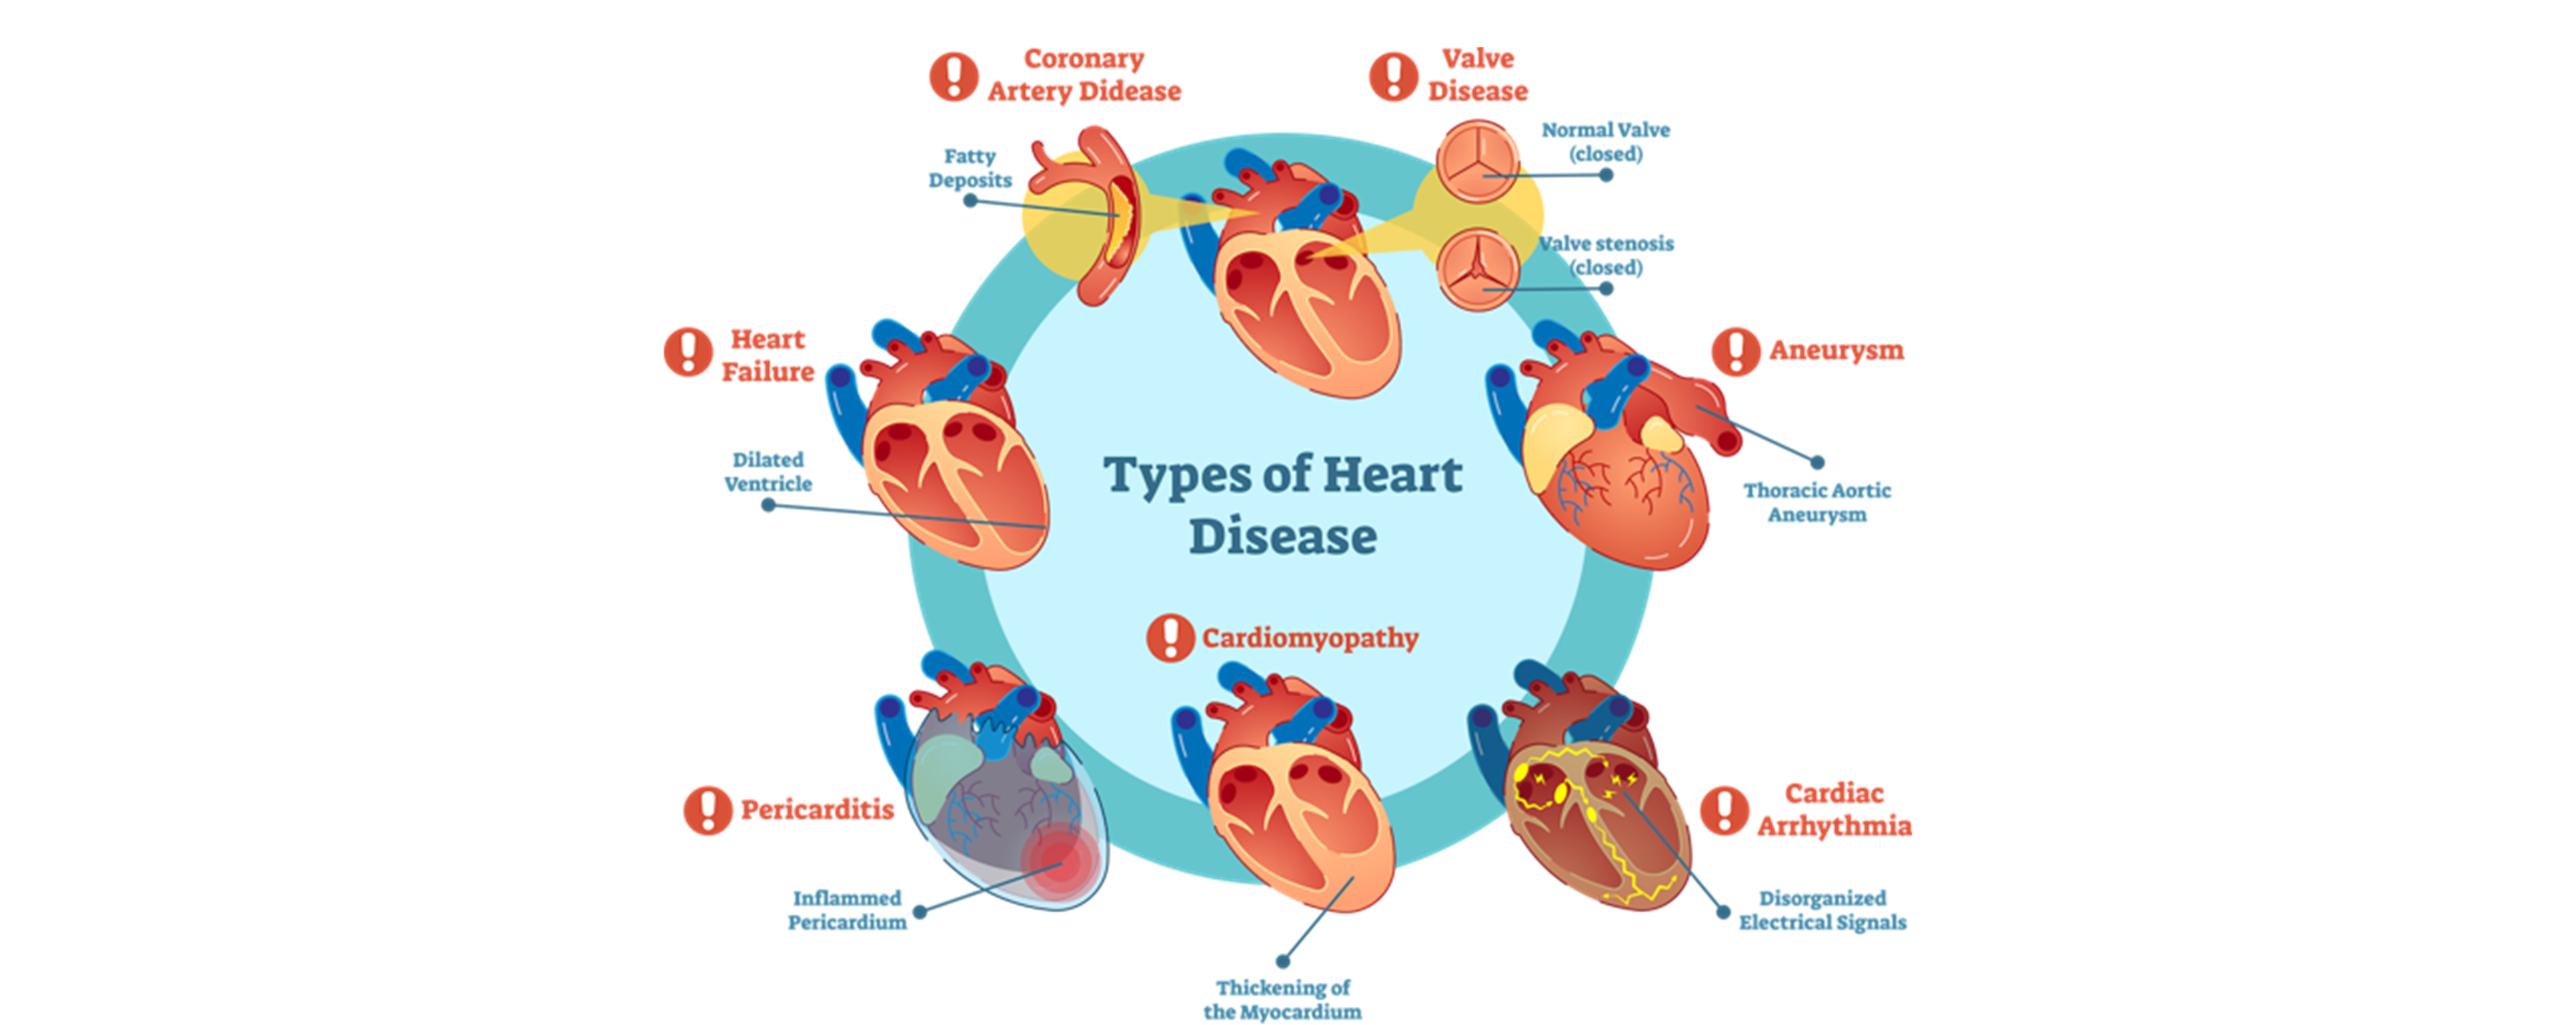
\includegraphics[width=1\textwidth]{Figures/Fig0.png}
    \caption{\bfseries\centering\fontsize{13pt}{0pt}\selectfont Heart disease}
    \label{fig1}
\end{figure} 

Figure \ref{fig1} shows some heart disease \cite{b1}.